\section{Introduction}
This open source project is about development of wireless data collecting equipment. The project is in cooperation with the geologist Dr .Andrew D. Wickert\cite{andrewWickert}, who has highly need for affordable and light-weighted field instrumentation for his research. He has develop Arduino-based low-power field environmental data logger\ref{fig:BottleLog}. He sought for assistance to Reykjavik University for help with development of communication module.

\begin{figure}
\centering
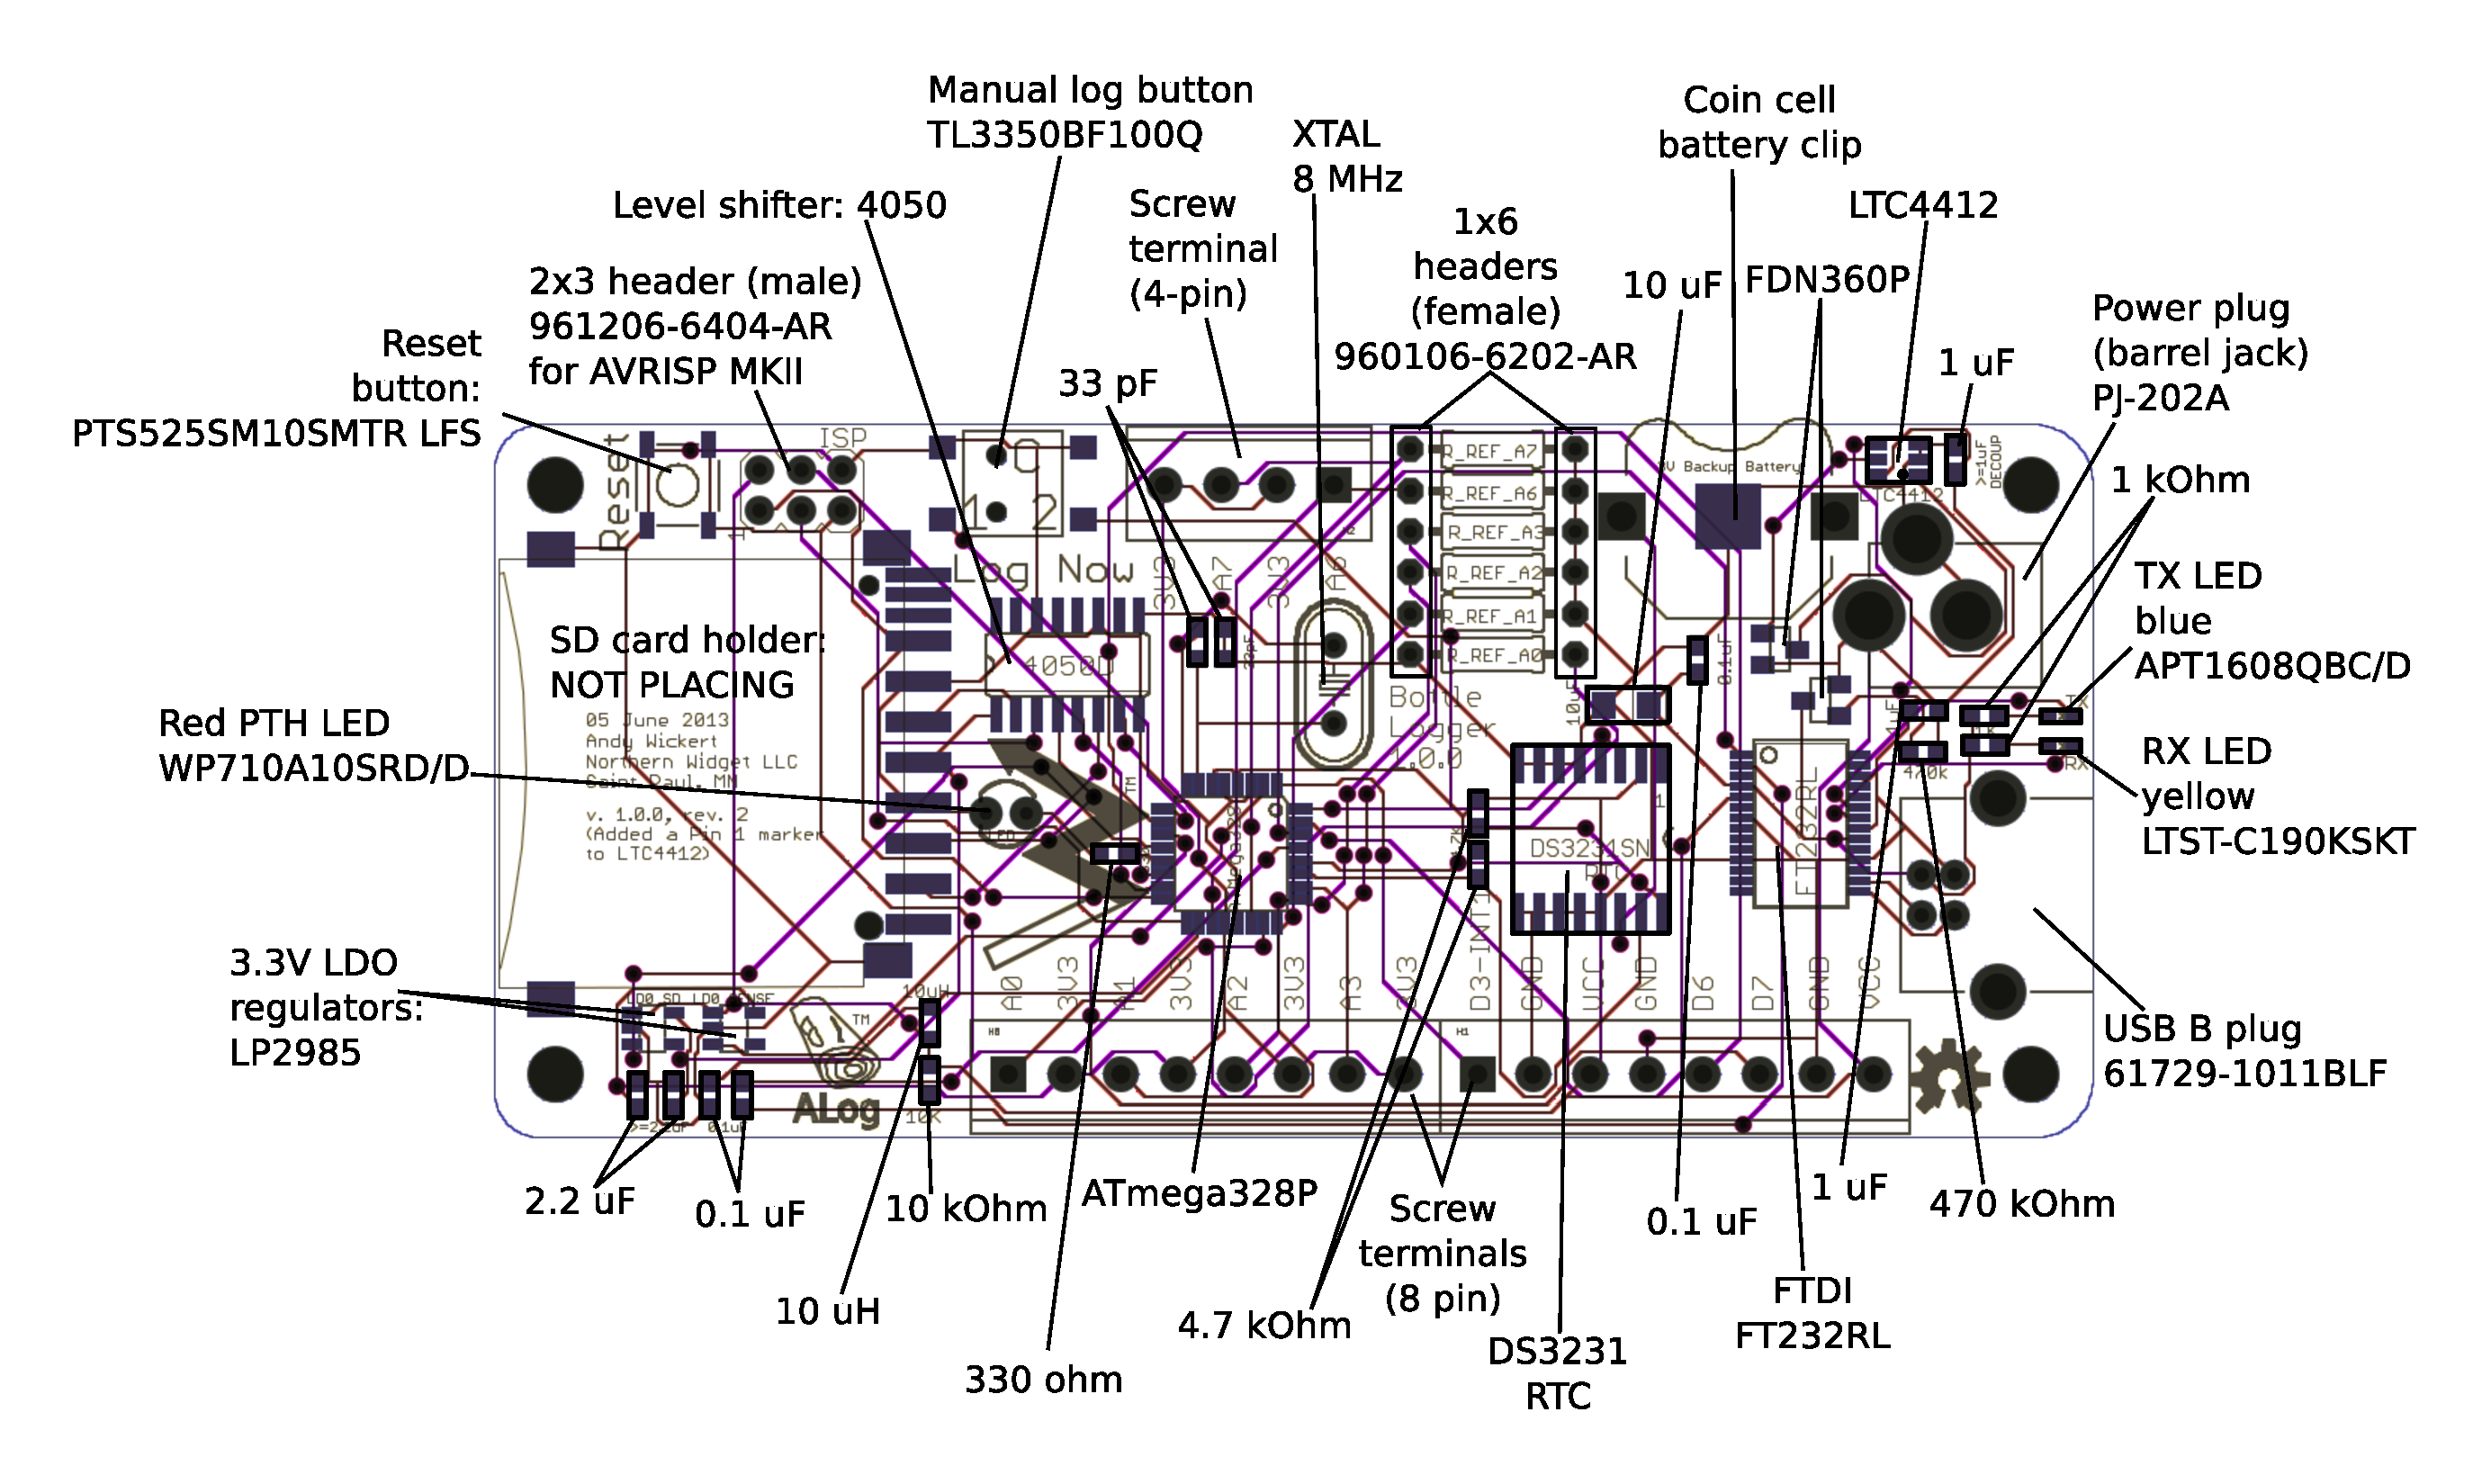
\includegraphics[height=5.7cm]{graphics/ALog_drawing.PDF}
\caption{Arduino-based low-power field environmental data logging platform: hardware schematics and circuit board layouts\label{fig:BottleLog}\cite{ALog-BottleLogger}}
\end{figure}

\subsection{Background}
Data sampling in nature is well know method to help scientist to understand its behavior. Back in days scientist had to sample data in real time on the field. Later on with automatic measurements equipment they could leave it behind in the field, then come back later and collect the data from them to process. With impact of communication technology the data collectors were able to sent data wireless in real time to scientist for processing. There are roughly 2 kinds of equipments available to day. Long range with GSM network \ref{fig:a} \ref{fig:b} that cost about \$3000. Then there are cheaper equipments around \$500 \ref{fig:c} \ref{fig:d} but the downfall is limited wireless range to 300 m.

\begin{figure}[H]
  \centering
  \subfloat[Cost \$3500\label{fig:a}\cite{WeatherShop2014}]
  {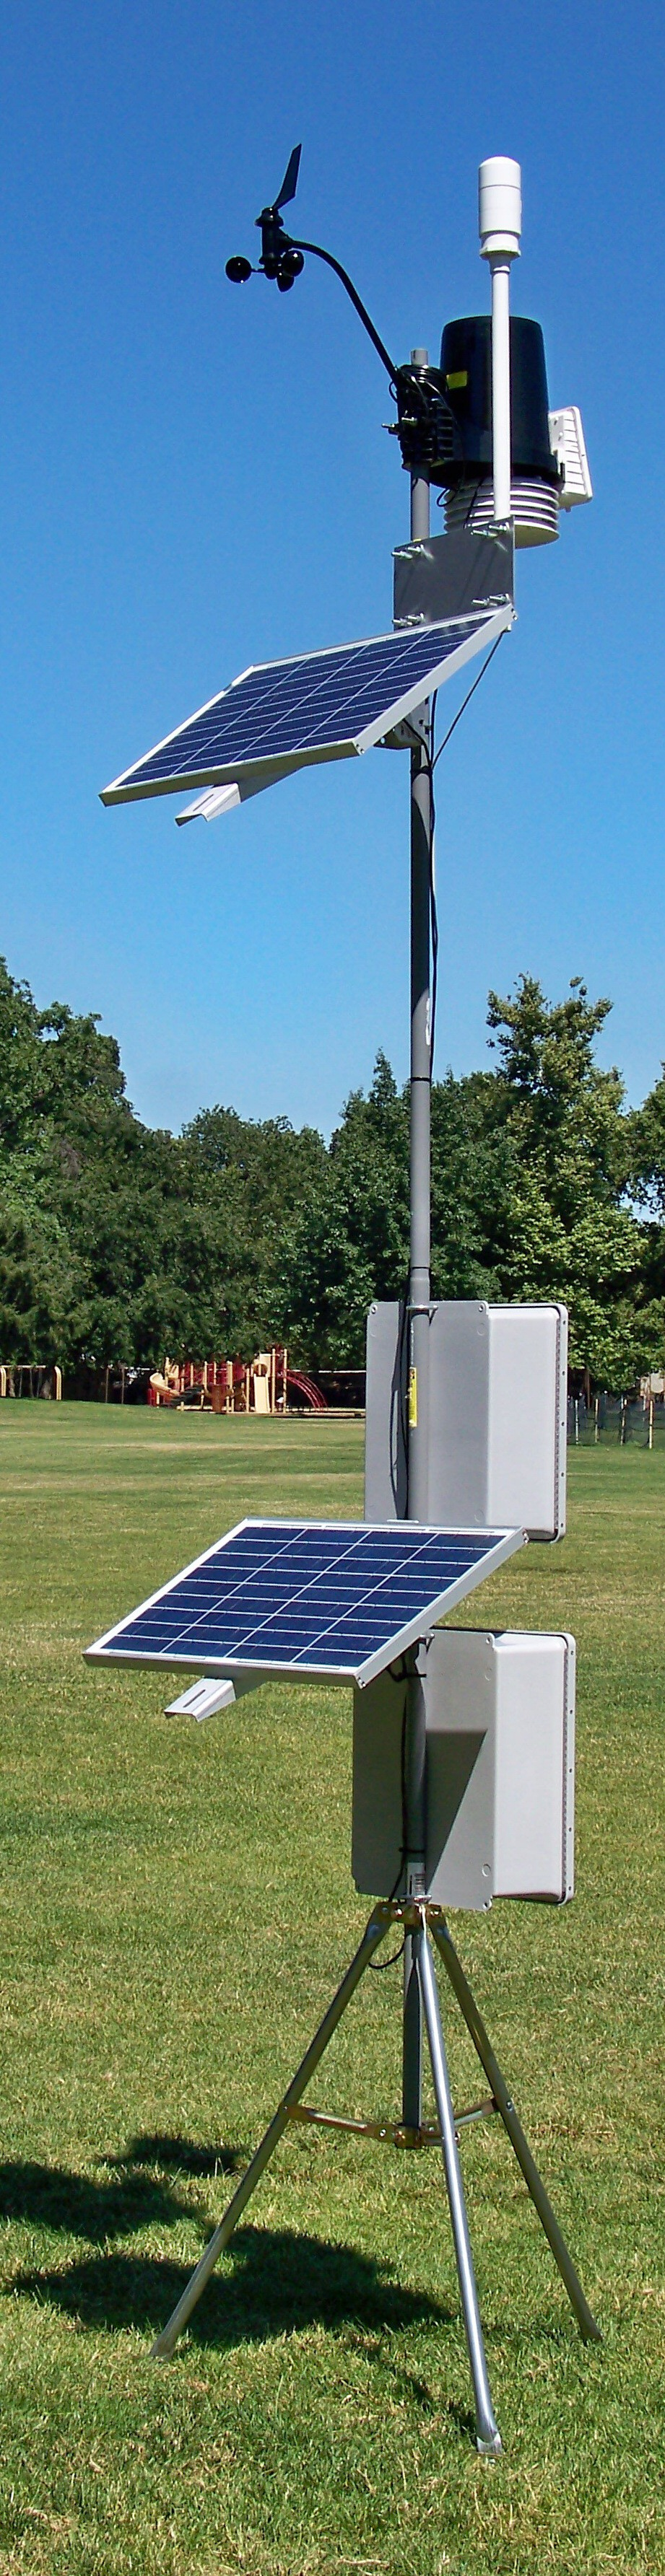
\includegraphics[height=5cm]{graphics/cellular_weather_station}}\quad
  \subfloat[Cost \$2800\label{fig:b}\cite{TexasWeatherInstruments2014}]
  {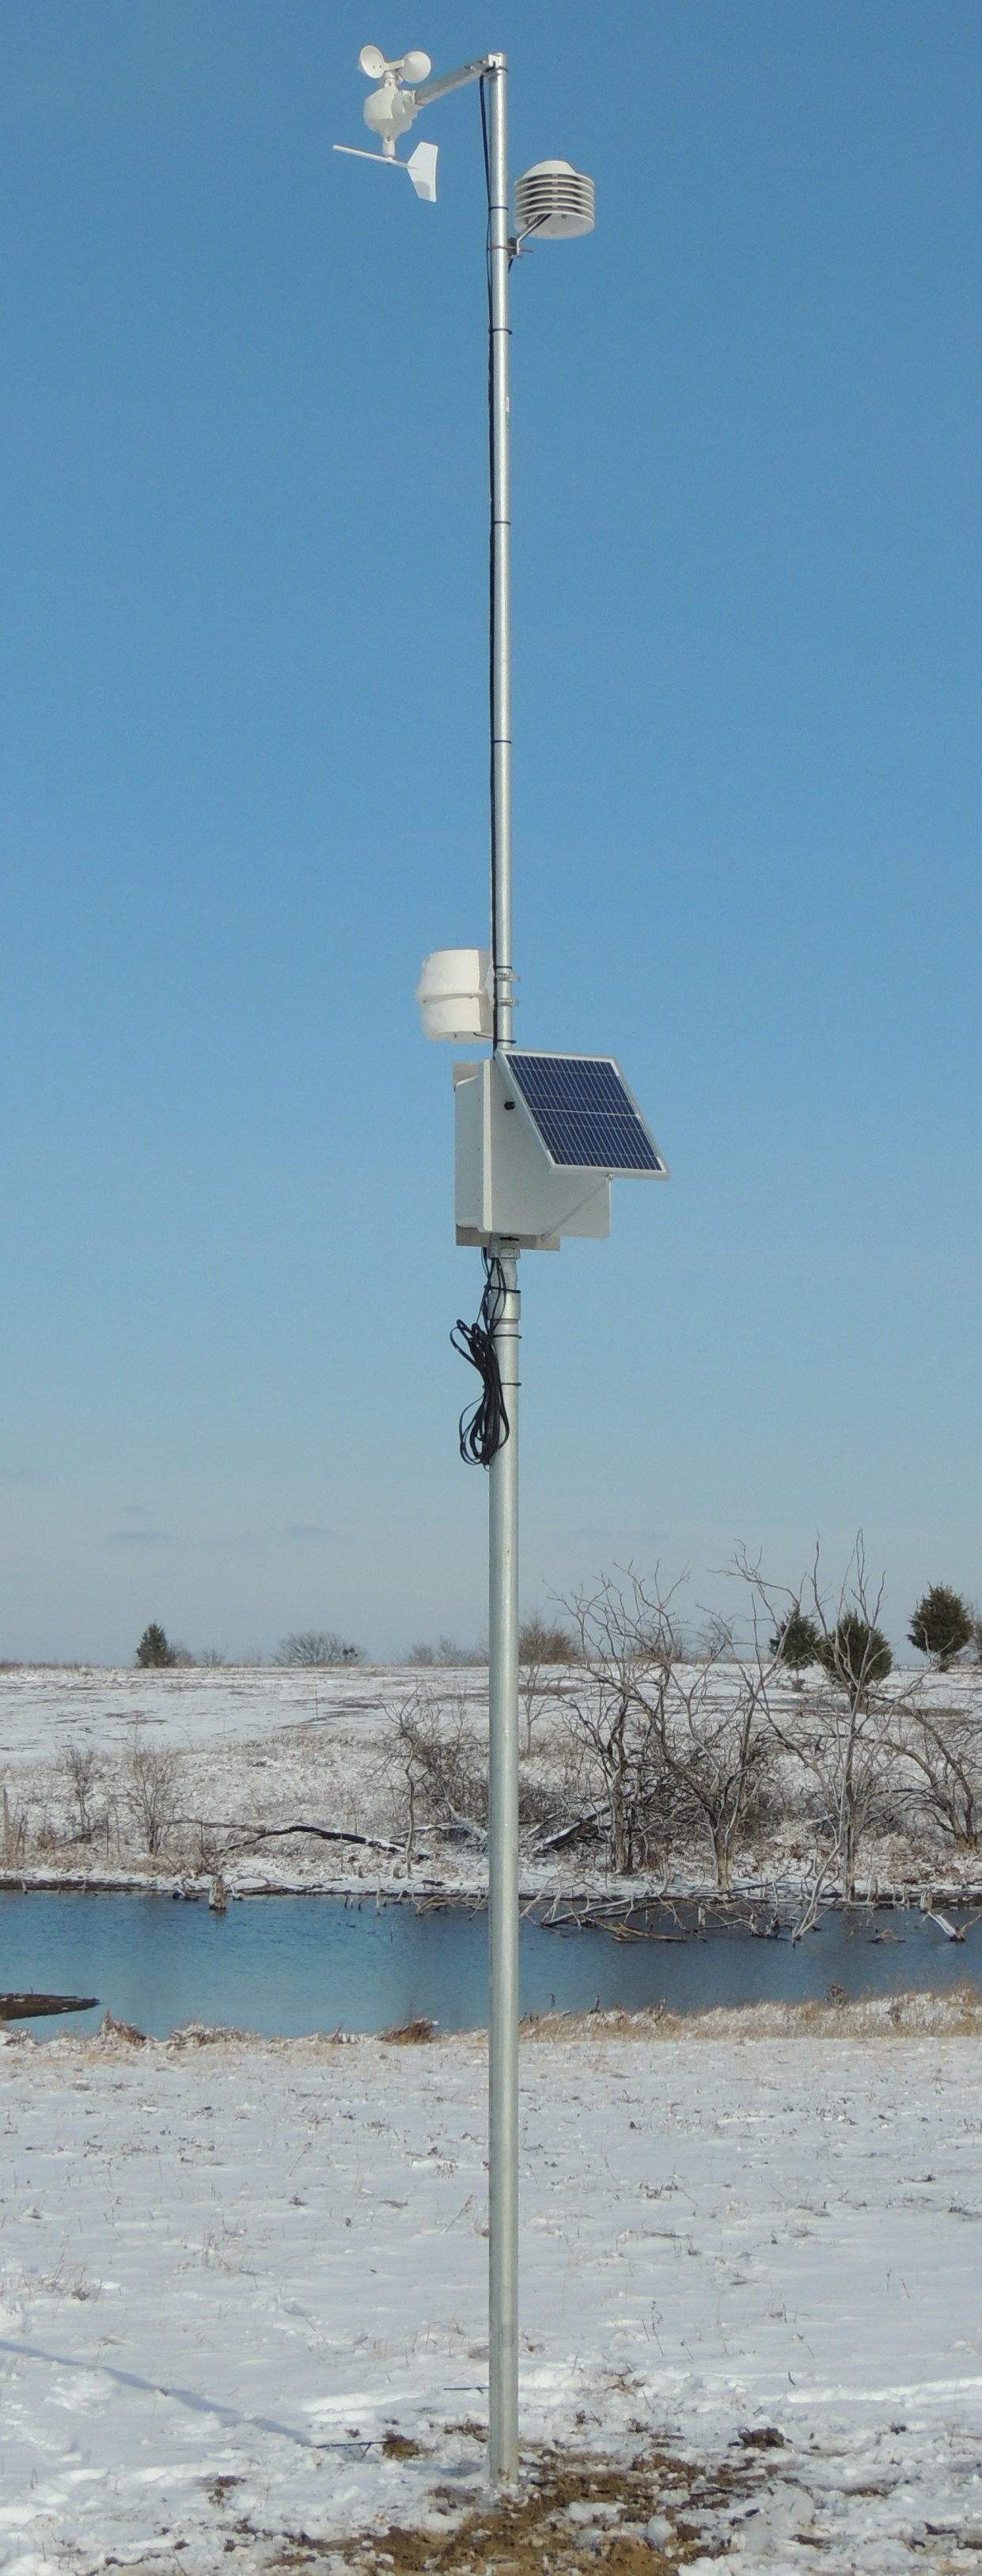
\includegraphics[height=5cm]{graphics/RWS-Snow}}\quad
  \subfloat[Cost \$658\label{fig:c}\cite{Scientific2014}]
  {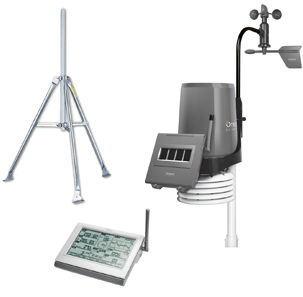
\includegraphics[height=3cm]{graphics/Oregon_Scientific_Pro_weather_system}}\quad
  \subfloat[Cost \$595\label{fig:d}\cite{Davis2014}]
  {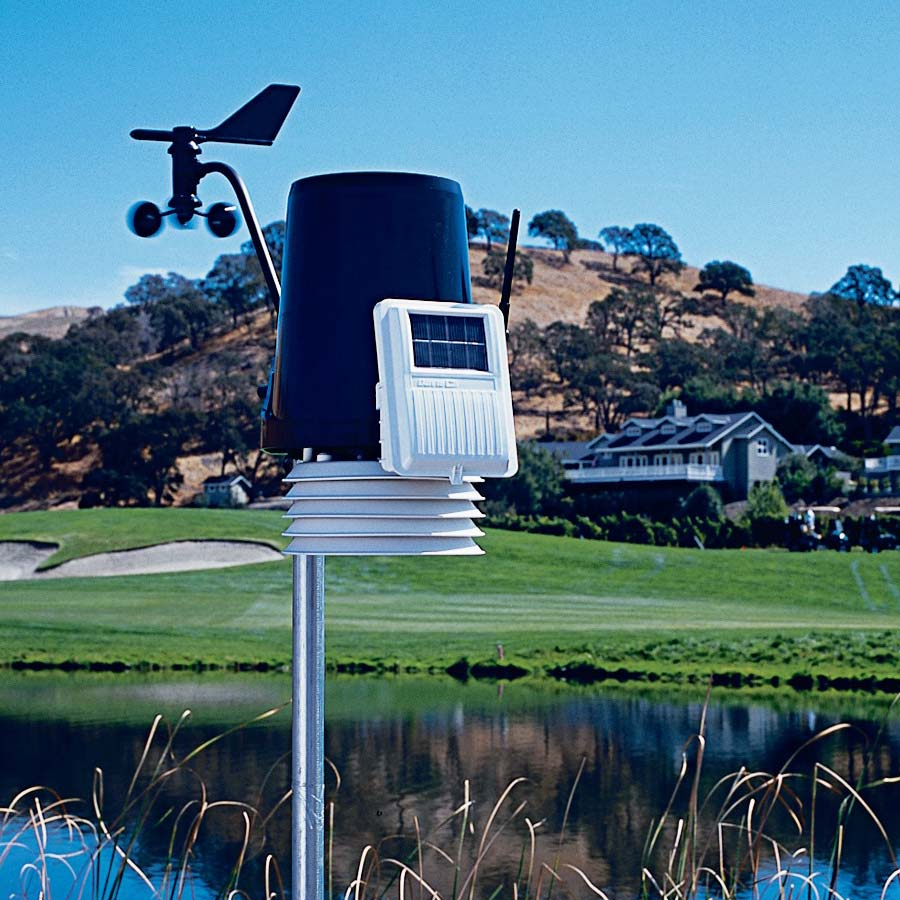
\includegraphics[height=3cm]{graphics/Davis_Vantage_Pro_2}}  
  \caption{Various price of weather stations}
  \label{fig:1}
\end{figure}

With that in mind the concept in the project is to make long-range communication data logger that are affordable. That factor is essential for scientific communities were budget can be limited. Another avenges is the possibility to get multiple equipments on the field for more dens coverage. 

\subsection{Requirements}
\textit{The requirments for this project are:}\\
FR1 Collect measurable data.\\
FR2 Store the data local.\\
FR3 Keeps data for x time.\\
FR4 Runs on own power source.\\
FR5 IP67 proof.\\
FR6 Sent data wireless through GSM network.\\
FR7 Store data on server.\\
FR8 Modular Design.\\
\\
DP1 Get temperature with TMP36 sensor.\\
DP2 Write temperature values to Arduino EEPROM.\\
DP3 Arduino MEGA has 4kB of EEPROM.\\
DP4 Have battery pack and minimize power consumption.\\
DP5 Fit all hardware into IP67 fiber box.\\
DP6 Send Jason formated data trough GSM shield.\\
DP7 Setup HTTP API server.\\
DP8 Well planed software design architecture.\\
\\
The most challenging requirements in the project is the software design. It's very critical to make the hole project modular. Solution to that is decrepit in DP7. Additionally there were added 3x wireless-sensor module to expand the coverage of the mother-base. They use Pololu Wixel to communicate to mother-base. Then the mother-base sample data from them and sent through GSM network to HTTP server.

